\whiteBGstarBegin
\setcounter{section}{0}
\section{Trắc nghiệm}
\begin{enumerate}[label=\bfseries Câu \arabic*:]
	
	
	\item \mkstar{1}
	
	\cauhoi
	{Công thức xác định độ lớn cường độ điện trường gây ra bởi điện tích $Q<0$ tại một điểm trong chân không, cách điện tích $Q$ một khoảng $r$ là
		\begin{mcq}(2)
			\item $E=9\cdot10^9 \dfrac{Q}{r^2}$.
			\item $E=-9\cdot10^9 \dfrac{Q}{r^2}$.
			\item $E=9\cdot10^9 \dfrac{Q}{r}$.
			\item $E=-9\cdot10^9 \dfrac{Q}{r}$.
		\end{mcq}
		
	}
	\loigiai
	{	\textbf{Đáp án: A.}
		
		Độ lớn cường độ điện trường gây ra bởi điện tích $Q$ tại một điểm cách $Q$ khoảng $r$ là
		$$E=9\cdot10^9 \dfrac{Q}{r^2}.$$
	}
	\item \mkstar{1}
	
	\cauhoi
	{Câu phát biểu nào sau đây \textbf{chưa đúng}?
		\begin{mcq}
			\item Qua mỗi điểm trong điện trường chỉ vẽ được một đường sức.
			\item Các đường sức của điện trường không cắt nhau.
			\item Đường sức của điện trường bao giờ cũng là đường thẳng.
			\item Đường sức của điện trường tĩnh không khép kín.
		\end{mcq}
		
	}
	\loigiai
	{	\textbf{Đáp án: C.}
		
		Đường sức của điện trường còn có thể là đường cong.
	}
	\item \mkstar{2}
	
	\cauhoi
	{Cường độ điện trường do điện tích $+Q$ gây ra tại điểm A cách nó một khoảng $r$ có độ lớn $E$. Nếu thay bằng điện tích $-2Q$ và giảm khoảng cách còn một nửa thì cường độ điện trường có độ lớn là
		\begin{mcq}(4)
			\item $8E$.
			\item $4E$.
			\item $\SI{0.25}{}E$.
			\item $E$.
		\end{mcq}
		
	}
	\loigiai
	{	\textbf{Đáp án: A.}
		
		Độ lớn cường độ điện trường lúc đầu:
		$$E=k \dfrac{|Q|}{r^2}.$$
		
		Độ lớn cường độ điện trường lúc sau:
		$$E'=k \dfrac{|-2Q|}{\frac{r^2}{4}}.$$
		
		Vậy
		$$\dfrac{E}{E'} = \dfrac{1}{2\cdot\frac{1}{4}} = \dfrac{1}{8} \Rightarrow E'=8E.$$
	}
	\item \mkstar{2}
	
	\cauhoi
	{Cường độ điện trường tạo bởi một điện tích điểm cách nó $\SI{2}{cm}$ bằng $\SI{e5}{V/m}$. Tại vị trí cách điện tích này bao nhiêu thì cường độ điện trường bằng $\SI{4e5}{V/m}$?
		\begin{mcq}(4)
			\item 2 cm.
			\item 1 cm.
			\item 4 cm.
			\item 5 cm.
		\end{mcq}
		
	}
	\loigiai
	{	\textbf{Đáp án: B.}
		
		Ta có $\dfrac{E}{E'} = \dfrac{1}{4} = \dfrac{r'^2}{r^2}$, suy ra:
		$$\dfrac{1}{2} = \dfrac{r'}{4} \Rightarrow r'=\SI{1}{cm}.$$
	}
	\item \mkstar{2}
	
	\cauhoi
	{Tại điểm A trong một điện trường, vectơ cường độ điện trường có hướng thẳng đứng từ trên xuống, độ lớn bằng $\SI{5}{V/m}$ có đặt điện tích $q=\SI{-4e-6}{C}$. Lực tác dụng lên điện tích $q$ có
		\begin{mcq}
			\item độ lớn bằng $\SI{2e-5}{N}$, hướng thẳng đứng từ trên xuống.
			\item độ lớn bằng $\SI{2e-5}{N}$, hướng thẳng đứng từ dưới lên.
			\item độ lớn bằng $\SI{2}{N}$, hướng thẳng đứng từ trên xuống.
			\item độ lớn bằng $\SI{4e-6}{N}$, hướng thẳng đứng từ dưới lên.
		\end{mcq}
		
	}
	\loigiai
	{	\textbf{Đáp án: B.}
		
		Do $q<0$ nên $\vec E$ cùng phương, ngược chiều với $\vec F$. Vậy $\vec F$ hướng thẳng đứng từ dưới lên. Độ lớn:
		$$F=|q|E = \SI{2e-5}{N}.$$
	}
	\item \mkstar{2}
	
	\cauhoi
	{Cường độ điện trường tạo bởi một điện tích điểm cách nó 4 cm bằng $\SI{e5}{V/m}$. Tại vị trí cách điện tích này bao nhiêu thì cường độ điện trường bằng $\SI{4e5}{V/m}$?
		\begin{mcq}(4)
			\item 2 cm.
			\item 1 cm.
			\item 4 cm.
			\item 5 cm.
		\end{mcq}
		
	}
	\loigiai
	{	\textbf{Đáp án: A.}
		
		Lập tỉ lệ:
		$$\dfrac{E_1}{E_2} = \dfrac{r_2^2}{r_1^2} \Rightarrow r_2 = \SI{2}{cm}.$$
	}
	\item \mkstar{2}
	
	\cauhoi
	{Cho một hình thoi tâm O, cường độ điện trường tại O triệt tiêu khi tại 4 đỉnh của hình thoi ta đặt
		\begin{mcq}
			\item các điện tích cùng độ lớn.
			\item các điện tích cùng dấu.
			\item các điện tích đối diện nhau cùng dấu, cùng độ lớn.
			\item các điện tích ở liền kề nhau khác dấu nhau.
		\end{mcq}
		
	}
	\loigiai
	{	\textbf{Đáp án: C.}
		
		Cho một hình thoi tâm O, cường độ điện trường tại O triệt tiêu khi tại 4 đỉnh của hình thoi ta đặt các điện tích đối diện nhau cùng dấu, cùng độ lớn.
	}
	\item \mkstar{2}
	
	\cauhoi
	{Tại một điểm xác định trong điện trường tĩnh, nếu độ lớn của điện tích thử tăng 2 lần thì độ lớn cường độ điện trường
		\begin{mcq}(2)
			\item tăng 2 lần.
			\item giảm 2 lần.
			\item không đổi.
			\item giảm 4 lần.
		\end{mcq}
		
	}
	\loigiai
	{	\textbf{Đáp án: C.}
		
		Cường độ điện trường không phụ thuộc vào điện tích thử nên nó không đổi.
	}
	\item \mkstar{2}
	
	\cauhoi
	{Đặt một điện tích dương, khối lượng không đáng kể vào một điện trường đều. Điện tích sẽ chuyển động
		\begin{mcq}
			\item dọc theo chiều của đường sức điện.
			\item ngược chiều với chiều của đường sức điện.
			\item vuông góc với các đường sức điện.
			\item tròn trong điện trường.
		\end{mcq}
		
	}
	\loigiai
	{	\textbf{Đáp án: A.}
		
		Điện tích dương chuyển động đến nơi tích điện âm, mà điện trường hướng từ nơi tích điện dương sang âm, nên điện tích dương chuyển động dọc theo chiều của đường sức điện.
	}
	\item \mkstar{2}
	
	\cauhoi
	{Yếu tố nào sau đây \textbf{không} ảnh hưởng đến cường độ điện trường tại điểm M gây ra bởi điện tích $Q$? Biết rằng tại M ta đặt một điện tích thử $q$.
		\begin{mcq}(2)
			\item Điện tích $Q$.
			\item Điện tích $q$.
			\item Khoảng cách từ $Q$ đến $q$.
			\item Hằng số điện môi.
		\end{mcq}
		
	}
	\loigiai
	{	\textbf{Đáp án: B.}
		
		Cường độ điện truòng tại một điểm không phụ thuộc vào điện tích thử $q$ đặt tại điểm đó.
	}
	\item \mkstar{2}
	
	\cauhoi
	{Một điện tích điểm $Q=\SI{-2e-7}{C}$ đặt tại điểm A trong môi trường có hằng số điện môi $\varepsilon =2$. Vectơ cường độ điện trường $\vec E$ do điện tích $Q$ gây ra tại điểm B có đặc điểm là (cho $\text{AB} = \SI{6}{cm}$)
		\begin{mcq}
			\item chiều từ A đến B, độ lớn $\SI{2.5e5}{V/m}$.
			\item chiều từ B đến A, độ lớn $\SI{2.5e5}{V/m}$.
			\item chiều từ A đến B, độ lớn $\SI{1.5e5}{V/m}$.
			\item chiều từ B đến A, độ lớn $\SI{1.5e5}{V/m}$.
		\end{mcq}
		
	}
	\loigiai
	{	\textbf{Đáp án: B.}
		
		Vì $Q$ là điện tích âm nên $\vec E$ hướng về phía $Q$ (từ B đến A) và có độ lớn:
		$$E=k \dfrac{|Q|}{\varepsilon r^2} = \SI{2.5e5}{V/m}.$$
	}
	\item \mkstar{2}
	
	\cauhoi
	{Hai điện tích gồm $q_1=\SI{2e-6}{C}$ và $q_2=\SI{-8e-6}{C}$ lần lượt đặt tại hai điểm A và B cách nhau 10 cm. Xác định điểm M trên đường thẳng AB mà tại đó có $\vec E_2 = 4 \vec E_1$.
		\begin{mcq}(2)
			\item M nằm trong AB với $\text{AM} = \SI{2.5}{cm}$.
			\item M nằm trong AB với $\text{AM} = \SI{5}{cm}$.
			\item M nằm ngoài AB với $\text{AM} = \SI{2.5}{cm}$.
			\item M nằm ngoài AB với $\text{AM} = \SI{5}{cm}$.
		\end{mcq}
		
	}
	\loigiai
	{	\textbf{Đáp án: B.}
		
		Về độ lớn, vì $|q_2| = 4 |q_1|$ nên để $\vec E_2 = 4 \vec E_1$ thì $r_2 = 4r_1$, do đó $\text{AM} = \text{BM} = \SI{5}{cm}$.
	}
	\item \mkstar{2}
	
	\cauhoi
	{Cho hai bản kim loại phẳng đặt song song tích điện trái dấu, thả không vận tốc đầu một electron vào điện trường giữa hai bản kim loại trên. Bỏ qua tác dụng của trọng trường. Quỹ đạo của electron là
		\begin{mcq}
			\item đường thẳng song song với các đường sức điện.
			\item đường thẳng vuông góc với các đường sức điện.
			\item một phần của đường parabol.
			\item một đường tròn.
		\end{mcq}
		
	}
	\loigiai
	{	\textbf{Đáp án: A.}
		
		Electron chuyển động ngược chiều điện trường, do đó quỹ đạo của electron là đường thẳng song song với các đường sức điện.
	}
	\item \mkstar{2}
	
	\cauhoi
	{Hai điện tích điểm $q_1$ và $q_2$ đặt tại hai điểm cố định A và B. Tại điểm M trên đoạn thẳng AB và gần A hơn, người ta thấy cường độ điện trường tổng hợp tại đó bằng 0. Kết luận nào sau đây đúng?
		\begin{mcq}
			\item $q_1$ và $q_2$ trái dấu, độ lớn $|q_1| > |q_2|$.
			\item $q_1$ và $q_2$ cùng dấu, độ lớn $|q_1| > |q_2|$.
			\item $q_1$ và $q_2$ trái dấu, độ lớn $|q_1| < |q_2|$.
			\item $q_1$ và $q_2$ cùng dấu, độ lớn $|q_1| < |q_2|$.
		\end{mcq}
		
	}
	\loigiai
	{	\textbf{Đáp án: D.}
		
		Để điểm M trên đoạn AB và gần A hơn có cường độ điện trường tổng hợp bằng 0 thì $q_1$ và $q_2$ cùng dấu, độ lớn $|q_1| < |q_2|$.
	}
	\item \mkstar{2}
	
	\cauhoi
	{Một điện tích điểm $Q$ dương trong chân không gây ra tại điểm M cách nó một khoảng $r=\SI{30}{cm}$ một điện trường có cường độ $E=\SI{40000}{V/m}$. Độ lớn điện tích $Q$ là
		\begin{mcq}(4)
			\item $Q=\SI{3e-8}{C}$.
			\item $Q=\SI{4e-7}{C}$.
			\item $Q=\SI{3e-6}{C}$.
			\item $Q=\SI{3e-5}{C}$.
		\end{mcq}
		
	}
	\loigiai
	{	\textbf{Đáp án: B.}
		
		Độ lớn điện tích $Q$ là
		$$E=k \dfrac{|Q|}{r^2} \Rightarrow Q = \SI{4e-7}{C}.$$
	}
	\item \mkstar{3}
	
	\cauhoi
	{Quả cầu nhỏ khối lượng $m=\SI{25}{g}$, mang điện tích $q=\SI{2.5e-7}{C}$ được treo bởi một sợi dây không dãn, khối lượng không đáng kể và đặt trong một điện trường đều với cường độ điện trường có phương nằm ngang, độ lớn $E=\SI{e6}{V/m}$. Góc lệch của dây treo so với phương thẳng đứng là
		\begin{mcq}(4)
			\item $30^\circ$.
			\item $45^\circ$.
			\item $60^\circ$.
			\item $75^\circ$.
		\end{mcq}
		
	}
	\loigiai
	{	\textbf{Đáp án: B.}
		
		Với quả cầu tích điện treo trong điện trường đều có phương nằm ngang, ta có:
		$$\tan \varphi = \dfrac{F}{P} = \dfrac{qE}{mg} = 1.$$
		
		Suy ra $\alpha = 45^\circ$.
	}
	\item \mkstar{3}
	
	\cauhoi
	{Cho hai điện tích điểm nằm ở hai điểm A và B có cùng dấu, cùng độ lớn. Điểm mà tại đó có cường độ điện trường tổng hợp bằng 0 là
		\begin{mcq}
			\item trung điểm của đoạn AB.
			\item tất cả các điểm trên đường trung trực của AB.
			\item những điểm tạo với A và B thành một tam giác đều.
			\item những điểm tạo với A và B thành một tam giác vuông cân.
		\end{mcq}
		
	}
	\loigiai
	{	\textbf{Đáp án: A.}
		
		Hai điện tích cùng dấu, cùng độ lớn thì tại trung điểm của đoạn thẳng nối hai điện tích sẽ có cường độ điện trường tổng hợp bằng 0.
	}
	\item \mkstar{3}
	
	\cauhoi
	{Hai điện tích điểm $q_1=\SI{-9}{\micro C}$, $q_2=\SI{4}{\micro C}$ đặt lần lượt tại A và B. Có thể tìm thấy vị trí của điểm M mà tại đó cường độ điện trường tổng hợp bằng 0 trên
		\begin{mcq}
			\item đường trung trực của AB.
			\item đường thẳng AB, nằm ngoài đoạn AB, gần A hơn.
			\item đường thẳng AB, nằm ngoài đoạn AB, gần B hơn.
			\item đoạn thẳng AB.
		\end{mcq}
		
	}
	\loigiai
	{	\textbf{Đáp án: C.}
		
		Vì $q_1$ và $q_2$ trái dấu nên vị trí cường độ điện trường tổng hợp bằng 0 nằm trên đường thẳng AB và ở phía ngoài đoạn AB.
		
		Vì độ lớn $|q_1| > |q_2|$ nên điểm M nằm gần B hơn.
	}
	\item \mkstar{3}
	
	\cauhoi
	{Hai điện tích $q_1<0$ và $q_2>0$ với $|q_2| > |q_1|$ đặt tại hai điểm A và B như hình vẽ (I là trung điểm của đoạn AB).
		\begin{center}
			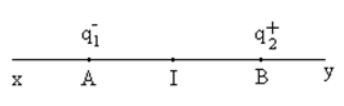
\includegraphics{../figs/VN11-2021-PH-TP004-1}
		\end{center}
	Điểm M mà tại đó cường độ điện trường tổng hợp bằng 0 nằm trên đoạn
		\begin{mcq}(4)
			\item AI.
			\item IB.
			\item B$y$.
			\item A$x$.
		\end{mcq}
		
	}
	\loigiai
	{	\textbf{Đáp án: D.}
		
		Vì $q_1$ và $q_2$ trái dấu nên vị trí cường độ điện trường tổng hợp bằng 0 nằm trên đường thẳng AB và ở phía ngoài đoạn AB.
		
		Vì độ lớn $|q_2| > |q_1|$ nên điểm M nằm gần A hơn.
	}
	\item \mkstar{4}
	
	\cauhoi
	{Một electron chuyển động dọc theo đường sức của một điện trường đều. Cường độ điện trường $E=\SI{100}{V/m}$. Vận tốc ban đầu của electron bằng $\SI{300}{km/s}$. Khối lượng của electron là $m=\SI{9.1e-31}{kg}$. Từ lúc bắt đầu chuyển động đến lúc vận tốc của electron bằng 0 thì electron đã chuyển động được đoạn đường là
		\begin{mcq}(2)
			\item $S=\SI{5.12}{mm}$.
			\item $S=\SI{2.56}{mm}$.
			\item $S=\SI{5.12e-3}{mm}$.
			\item $S=\SI{2.56e-3}{mm}$.
		\end{mcq}
		
	}
	\loigiai
	{	\textbf{Đáp án: B.}
		
		Gia tốc của electron trong điện trường:
		$$a=\dfrac{F}{m} = \dfrac{qE}{m} = \SI{1.76e13}{m/s^2}.$$
		
		Giá trị đại số: $a=\SI{-1.76e13}{m/s^2}$.
		
		Quãng đường chuyển động được:
		$$2aS = v^2 - v_0^2 = 0 - v_0^2 \Rightarrow S \approx \SI{2.56e-3}{m} \approx \SI{2.56}{mm}.$$
	}
\end{enumerate}

\whiteBGstarEnd

\loigiai
{
	\begin{center}
		\textbf{BẢNG ĐÁP ÁN}
	\end{center}
	\begin{center}
		\begin{tabular}{|m{2.8em}|m{2.8em}|m{2.8em}|m{2.8em}|m{2.8em}|m{2.8em}|m{2.8em}|m{2.8em}|m{2.8em}|m{2.8em}|}
			\hline
			1.A  & 2.C  & 3.A  & 4.B  & 5.B  & 6.A  & 7.C  & 8.C  & 9.A  & 10.B  \\
			\hline
			11.B  & 12.B  & 13.A  & 14.D  & 15.B  & 16.B  & 17.A  & 18.C  & 19.D  & 20.B  \\
			\hline
		\end{tabular}
	\end{center}
}
\section{Tự luận}
\begin{enumerate}[label=\bfseries Câu \arabic*:]
	\item \mkstar{1}
	
	\cauhoi{
		Hãy nêu khái niệm, công thức và đặc điểm về phương, chiều, độ lớn của cường độ điện trường.
	}
	
	\loigiai{
		
		Cường độ điện trường là đại lượng vật lý đặc trưng cho tác dụng mạnh hay yếu của điện trường tại một điểm.
		
		Công thức:
		$$\vec E = \dfrac{\vec F}{q}.$$
		
		\begin{itemize}
			\item Điểm đặt: đặt tại điểm đang xét;
			\item Phương: là đường thẳng nối giữa $Q$ và điểm đang xét;
			\item Chiều: hướng ra xa $Q$ nếu $Q$ dương, hướng vào $Q$ nếu $Q$ âm;
			\item Độ lớn: $E=\dfrac{F}{|q|}$, tuy nhiên $E$ không phụ thuộc vào điện tích $q$.
		\end{itemize}
	}
	
	\item \mkstar{2}
	
	\cauhoi{
		Phát biểu nguyên lý chồng chất điện trường. Xác đinh độ lớn của vectơ cường độ điện trường tổng hợp trong các trường hợp sau:
		\begin{enumerate}
			\item $\vec E_1$ cùng phương, cùng chiều với $\vec E_2$;
			\item $\vec E_1$ cùng phương, ngược chiều với $\vec E_2$;
			\item $\vec E_1$ vuông góc với $\vec E_2$;
			\item $\vec E_1$ hợp với $\vec E_2$ một góc $\alpha$ bất kì.
		\end{enumerate}
	}
	
	\loigiai{
		
		Nếu tại một điểm dưới tác dụng của nhiều điện trường $\vec E_1$, $\vec E_2$, $\vec E_3$, $\ldots$ do các điện tích $q_1$, $q_2$, $q_3$, $\ldots$ gây ra thì cường độ điện trường tổng hợp tại đó là
		$$\vec E = \vec E_1 + \vec E_2 + \vec E_3 + \ldots + \vec E_n.$$
		
		Các trường hợp đặc biệt:
		\begin{enumerate}
			\item $\vec E_1$ cùng phương, cùng chiều với $\vec E_2$;
			
			$$E=E_1 + E_2$$
			\item $\vec E_1$ cùng phương, ngược chiều với $\vec E_2$;
			
			$$E=E_1 - E_2$$
			\item $\vec E_1$ vuông góc với $\vec E_2$;
			
			$$E=\sqrt{E_1^2 + E_2^2}$$
			\item $\vec E_1$ hợp với $\vec E_2$ một góc $\alpha$ bất kì.
			
			$$E=\sqrt{E_1^2 + E_2^2 + 2E_1 E_2 \cos \alpha}$$
		\end{enumerate}
		
	}
	\item \mkstar{3}
	
	\cauhoi{
		Một điện tích điểm $q=\SI{e-7}{C}$ đặt tại điểm M trong điện trường do một điện tích điểm $Q$ gây ra và chịu tác dụng của một lực là $F=\SI{3e-3}{N}$.
		\begin{enumerate}
			\item Tính cường độ điện trường do $Q$ gây ra tại điểm M;
			\item Nếu điểm M cách $Q$ một đoạn 30 cm, hãy xác định độ lớn của $Q$.
		\end{enumerate}
	}
	
	\loigiai{
			\begin{enumerate}
			\item Tính cường độ điện trường do $Q$ gây ra tại điểm M;
			$$E_\text{M} = \dfrac{F}{q} = \SI{3e4}{V/m}$$
			\item Nếu điểm M cách $Q$ một đoạn 30 cm, hãy xác định độ lớn của $Q$.
			$$E_\text{M} = k \dfrac{|Q|}{r_\text{M}^2} \Rightarrow |Q|=\dfrac{E_\text{M}r_\text{M}^2}{k} = \SI{3e-7}{C}$$
		\end{enumerate}
		
	}
	\item \mkstar{4}
	
	\cauhoi{
		Tại ba đỉnh của một tam giác ABC vuông tại A, các cạnh $\text{BC} = \SI{50}{cm}$, $\text{AC} = \SI{40}{cm}$, $\text{AB} = \SI{30}{cm}$ ta đặt các điện tích $q_1 = q_2 = q_3 = \SI{e-9}{C}$. Xác định cường độ điện trường tại H với H là chân đường cao kẻ từ A.
	}
	
	\loigiai{
		\begin{center}
			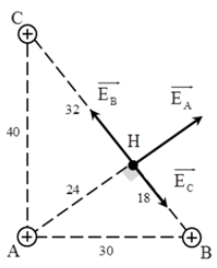
\includegraphics{../figs/VN11-2021-PH-TP004-3}
		\end{center}
	
	Ta có: $\text{HC} = \SI{32}{cm}$, $\text{HB} = \SI{18}{cm}$, $\text{AH} = \SI{24}{cm}$.
	
	Cường độ điện trường gây ra tại H có chiều như hình vẽ trên, về độ lớn:
	$$E_\text{H} = \sqrt{E_\text{A}^2 + (E_\text{B} - E_\text{C})^2} \approx \SI{246}{V/m}.$$
		
	}
	\item \mkstar{4}
	
	\cauhoi{
		Cường độ điện trường của một điện tích phụ thuộc vào khoảng cách $r$ được mô tả như đồ thị dưới đây.
		\begin{center}
			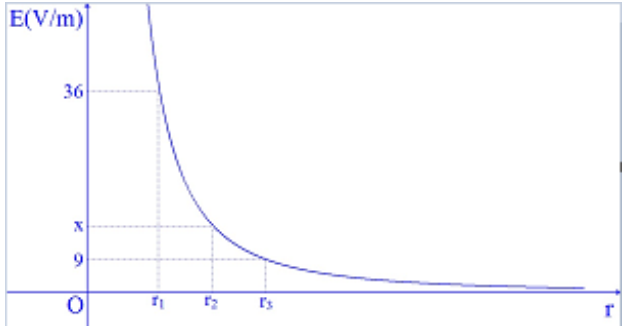
\includegraphics{../figs/VN11-2021-PH-TP004-2}
		\end{center}
	Biết $r_2=\dfrac{r_1+r_3}{2}$ và các điểm cùng nằm trên một đường sức. Tìm giá trị của $x$.
	}
	
	\loigiai{
		
		Ta có $r\sim \dfrac{1}{\sqrt{E}}$, mà $r_2 = \dfrac{r_1+r_3}{2}$ nên suy ra
		$$\dfrac{2}{\sqrt{E_2}} = \dfrac{1}{\sqrt{E_1}} + \dfrac{1}{\sqrt{E_3}} \Rightarrow E_2 = x = \SI{16}{V/m}.$$
	}
	
\end{enumerate}